% ==============================================================================
% Paid to Be Absent: Direction Compensation and Capacity Withholding
% in the South Australian Electricity Market
%
% Compile (from manuscript/): 3-pass XeLaTeX + BibTeX
%   xelatex -interaction=nonstopmode paper.tex
%   bibtex paper
%   xelatex -interaction=nonstopmode paper.tex
%   xelatex -interaction=nonstopmode paper.tex
%
% Bibliography: ../Bibliography_base.bib (repo root, single source)
% Exhibits: \input from ../output/tables/, figures from ../output/figures/
% ==============================================================================
\documentclass[12pt]{article}

\usepackage[margin=1in]{geometry}
\usepackage{amsmath, amssymb}
\usepackage{booktabs}
\usepackage{graphicx}
\usepackage{caption}
\usepackage{setspace}
\usepackage{natbib}
\usepackage{threeparttable}
\usepackage{adjustbox}
\usepackage[hidelinks]{hyperref}

\graphicspath{{../output/figures/}}
\bibliographystyle{plainnat}

\onehalfspacing
\captionsetup{font=small, labelfont=bf}

% --- Notation macros (single source of truth for symbols) ---
\newcommand{\dt}{d_t}                 % direction compensation price
\newcommand{\pex}{\mathit{pex}}       % rivals-only ex-ante essentiality flag
\newcommand{\cheap}{\mathit{cheap}}   % cheap-capacity share outcome

\title{Paid to Be Absent: Direction Compensation and Capacity Withholding
in the South Australian Electricity Market\thanks{Monash University.
Draft --- do not cite.}}
\author{Eric Liu}
\date{\today}

\begin{document}

\maketitle

\begin{abstract}
\noindent
When South Australia's electricity market leaves the grid short of synchronous
generation, the operator directs specific units to run and compensates them
for their entire directed output at a backward-looking reference price --- the
90th percentile of the trailing year of spot prices. Over 2022--2024 this
scheme paid three gas steam units \$141.9 million for directed output worth
\$7.2 million at spot. Using the complete bid ladder at five-minute
resolution, I show that the directed units' withholding co-varies with the
administered payment itself, on exactly the margin the payment operates:
the probability that a unit keeps its minimum-stable quantum within
dispatch's reach --- the act that averts a direction --- falls by 8.6
percentage points per \$100/MWh of compensation price on essential relative
to matched intervals (wild-cluster-bootstrap $p<0.01$; randomization
inference $p=0.046$; interpretation committed before estimation), while
offered depth conditional on that choice shows no response. Ordinary market
power assigns no role to this margin, and essential periods are measurably
more competitive than ordinary ones, so the market-power alternative fails
on the sign of its own conditions; the gap also held through nine months of
cheap fuel while the backward-looking formula still paid crisis rates,
though that timing contrast is marginal ($p=0.09$), so the cross-month
pattern is reported as consistent with payment-seeking rather than proof of
it. Mechanism
evidence locates the conduct in a standing absent posture rather than daily
calibration: directed output equals the units' operating floor, evening
exits are event-timed rather than need-timed, and an earlier day-grain
finding of state-dependent withdrawal is shown to be an artifact of bids
formed under direction. The conduct is a property of the mechanism's design --- a gross
payment at a stale scarcity price to units whose market alternative is
loss-making --- and each design defect maps to a standard repair.
\end{abstract}

\medskip
\noindent\textbf{Keywords:} electricity markets; capacity withholding;
out-of-market directions; compensation design; system security\\
\textbf{JEL codes:} L94; L51; D22; Q41

\clearpage

% ------------------------------------------------------------------------------
% §1 Introduction — drafted last, Phase C
% ------------------------------------------------------------------------------
\section{Introduction}\label{sec:intro}

When an electricity market cannot keep the lights on by itself, the system
operator reaches outside it: a \emph{direction} orders a generator to run for
system security, and a compensation rule decides what that order pays.
Between 2022 and 2024, South Australia's direction scheme paid three gas
steam units at Torrens Island \$141.9 million for directed output the energy
market valued at \$7.2 million --- twenty dollars through the direction
channel for every dollar of market value. This paper asks whether that
transfer was an unfortunate price for security, or whether the scheme's own
design induced the scarcity it paid to relieve. The evidence supports the
second reading: the units' capacity withholding responds to the size of the
administered compensation price itself --- a margin to which no ordinary
market-power story assigns any role.

The setting has three ingredients that together make it a clean laboratory
for studying how out-of-market payments shape in-market conduct. First, a
\emph{security requirement}: South Australia's renewables-dominated grid
needs a minimum set of synchronous machines online, and when market dispatch
leaves the set incomplete, the operator directs specific units online. Second, a
\emph{gross payment}: a directed unit is compensated for its entire directed
output at a regulated reference price --- measured in this paper's data,
compensation is $0.95 \times$ directed MWh $\times$ the reference price, with
$R^{2}=0.99$ --- regardless of what it would have earned otherwise. Third, a
\emph{backward-looking price}: the reference price is the 90th percentile of
the trailing year of spot prices, so the 2022 energy crisis mechanically
paid itself forward into 2023--2024, holding the payment near \$350/MWh while
fuel costs halved. A unit that is loss-making in the energy market --- spot
exceeded fuel cost in 3.9\% of directed intervals --- faces a stark
choice between committing capacity to a market that will not cover its costs
and being absent, essential, directed, and paid gross at last year's scarcity
price.

The paper's empirical object is the availability margin of conduct: the
share of registered capacity a unit offers at prices at which it could
actually run. Two questions structure the analysis. RQ1: do units withhold
more when they are \emph{essential} --- when no combination of rival units
satisfies the security requirement without them? RQ2, the identifying
question: conditional on essentiality, does withholding respond to the
\emph{size} of the compensation price? The distinction carries the
identification. Being essential bundles compensation-eligibility with
whatever ordinary market power comes with being needed, and both predict
withholding-when-essential. But ordinary market power is indifferent to the
compensation formula; payment-seeking is not. A dose response to the
administered price, specific to essential intervals, is a signature only the
payment channel produces.

The answers. On RQ1, the directed workhorse station withholds more when
essential ($-0.076$ of registered capacity, stable in sign across all 72
leave-one-month-out re-estimates), and a direct control for energy-market
competition absorbs essentially none of the response --- indeed the
market-power alternative fails on the sign of its own conditions, because
essential periods are measurably \emph{more} competitive than ordinary ones,
not tighter. On RQ2, the essential-versus-matched withholding gap widens by
5.1 percentage points of registered capacity per \$100/MWh of compensation
price (wild-cluster-bootstrap $p<0.01$ on both outcome definitions), an
estimate whose interpretation was committed before it was run, and stable
across every treatment of the June 2022 crisis month. Decomposing the
outcome sharpens the finding onto the margin the mechanism actually pays:
the entire response is the probability that the unit's minimum-stable
quantum is within dispatch's reach --- the self-commitment choice that
averts or invites a direction --- which falls by 8.6 percentage points per
\$100/MWh (randomization-inference $p=0.046$), while offered depth
conditional on that choice responds not at all. The causal reading is
disciplined by the formula's own timing: gas prices fell nine months before
the payment did, and the gap tracked the payment, not the fuel, through
that wedge --- though the sharpest such contrast rests on four months and
clears only the 10\% level, so this paper's claim for the cross-month
gradient is ``consistent with payment-seeking,'' stated exactly.

Mechanism evidence locates the conduct precisely. The absence is a
\emph{standing posture}, not a daily calibration: the units' day-ahead bids
withhold or price out their floor megawatts on 76--80\% of all cleanly
observed days, in multi-day blocks, organised as a rotating station roster
that never once --- in 73 opportunities --- declared less than the security
standard required. Day-level tests, their interpretations committed in
advance and run on bids formed
outside direction exposure, find the posture indifferent to the daily
security envelope (evening exits are event-timed, not need-timed) and to the
daily prize (the offered floor price does not move on essential days). What
the direction buys is presence: directed output equals the units' operating
floor, with 55.9\% of episodes delivering zero or negative excess energy
over it. And the
paper reports its own correction: an earlier day-grain finding of
state-dependent withdrawal ($-12.7$ points on essential days, $p<0.001$) was
a contamination artifact --- 54\% of essential days had bids formed while a
direction was running or pending --- and vanishes on clean days. What
survives decontamination is the standing posture, its gross payment, and the
cross-month dose response.

The paper contributes to three literatures. The empirical market-power
literature in electricity measures conduct on the pricing margin: markups
over marginal cost \citep{Wolfram1999_duopoly,
BorensteinBushnellWolak2002_california}, bidding in multi-unit auctions
against theoretical benchmarks \citep{vonderFehrHarbord1993_spot,
HortacsuPuller2008_ercot}, pivotal-supplier ability and incentive
\citep{Wolak2003_unilateral, McRaeWolak2014_unilateral}, and physical
withholding --- as an input to price manipulation
\citep{JoskowKahn2002_california} or disguised as plant failures
\citep{FogelbergLazarczyk2019_failures,
BerglerHeimHuschelrath2017_failures}. The conduct documented here operates
on a margin that the literature treats as exogenous --- whether capacity is
offered at all --- and responds to a price that appears in none of its
models: the administered compensation rate. The nearest analytical
neighbour is the inc-dec gaming literature, in which units position in the
energy market in anticipation of out-of-market redispatch payments
\citep{HirthSchlecht2020_incdec}; this paper supplies field evidence of
that mechanism's signature, in a setting where the payment rate moves
through a mechanical formula. Second, the out-of-market payments
literature: \citet{BushnellWolak1999_rmr} argued that the design of
California's reliability-must-run contracts created serious incentive
problems and distorted bidding, and \citet{TeirilaRitz2019_capacity}
document market power in an administered capacity auction; this paper
supplies the payment-gradient evidence that debate never had. Third, the
capacity-mechanism design literature
\citep{CramtonOckenfelsStoft2013_capacity, Fabra2018_capacity}: the episode
is a natural experiment in what happens when an availability payment is
grossed up, backward-indexed, and layered onto an energy-only market ---
the design pays for absence, and absence is what it gets. Against all
three, one innocent account deserves naming early: start-up costs and
unit-commitment frictions rationalise block-level absence for steam units
\citep{Reguant2014_complex}, and this paper's mechanism evidence is fully
consistent with commitment costs shaping the posture's \emph{form}. What
commitment costs cannot produce is the posture's \emph{price sensitivity}
--- there is no unit-commitment reason for the self-commitment margin to
track a compensation formula --- which is exactly the object the paper's
identifying tests isolate.

The findings' scope is stated as carefully as their content. Nothing here
establishes daily intent: in this system the weather clock and the direction
clock are the same clock, and a desk watching either looks identical. The
claim is about the mechanism, not the desk's state of mind --- under this
payment structure a standing absent posture dominates commitment across
essentially all conditions, so rational conduct converges on exactly what the
data show, whatever its motive. That is an indictment of the design, and the
design is the policy lever: Section~\ref{sec:discussion} maps each defect
(gross payment, backward-looking price, unpriced presence) to a standard
repair, and notes the epilogue --- in September 2025 the synchronous
requirement was cut to one unit, closing the regime this paper studies.

Section~\ref{sec:setting} details the institutions; Section~\ref{sec:data}
the data and their validation against the operator's published statistics;
Section~\ref{sec:descriptives} the descriptive anatomy of the scheme;
Section~\ref{sec:design} the outcome, the essentiality flag, and the two
specifications; Section~\ref{sec:results} the regression results;
Section~\ref{sec:mechanism} the mechanism evidence and the contamination
correction; Section~\ref{sec:robustness} robustness;
Section~\ref{sec:discussion} concludes with design implications.

% ------------------------------------------------------------------------------
% §2 Institutional setting — drafted Phase C from:
%   Direction_clean/README.md; findings_task1b.md (gross payment, post-fix);
%   F1/F2b readout; memory: project_sa_regime_exit_2025, project_aemo_qed_direction_cost
% ------------------------------------------------------------------------------
\section{Institutional Setting}\label{sec:setting}

\subsection{Directions in the National Electricity Market}

The Australian National Electricity Market (NEM) is an energy-only gross pool:
generators submit offer curves --- up to ten price bands with quantities revisable
until dispatch\footnote{Rebidding is regulated: since 2016, offers must not
be false or misleading and late rebids require contemporaneous records
\citep{AEMC2015_goodfaith}. The conduct studied in this paper operates
through availability declarations and band quantities, which are and remain
freely revisable.} --- and a security-constrained dispatch engine clears the market
every five minutes. South Australia is the NEM's high-renewables frontier. Wind
and rooftop solar routinely supply most of regional demand, and on sunny, windy
days the energy market has no commercial work for the state's gas-fired
synchronous generators.

The energy market clears energy; it does not clear system security. South
Australia's grid requires a minimum complement of synchronous machines online to
provide system strength and inertia, codified as a set of minimum synchronous
generator combinations that the Australian Energy Market Operator (AEMO) must
maintain. When market dispatch leaves the requirement unmet --- typically in
exactly those high-renewables, low-price periods --- AEMO issues a
\emph{direction}: an instruction to a specific generating unit to synchronise,
or to remain synchronised, outside the normal dispatch process. A direction
compels presence, not output. A directed unit must be online; it typically runs
at its minimum stable loading.\footnote{Section~\ref{sec:mechanism} measures
this directly: directed output equals the unit's operating floor almost
exactly, with 55.9\% of resolved direction episodes delivering zero or negative
output in excess of the floor block.}

\subsection{Compensation: a gross payment at a backward-looking reference price}

A directed participant is entitled to compensation under clause 3.15.7 of
the National Electricity Rules (NER), with the cost recovered from market
participants under clause 3.15.8 \citep{AEMC2024_ner}. The reference price --- the
\emph{compensation price} $\dt$ throughout this paper --- is the 90th percentile
of South Australian spot prices over the trailing 365 days. Three design features
matter for everything that follows.

First, the payment is effectively \emph{gross}: compensation tracks the unit's
entire directed output valued at $\dt$, not the increment over what the unit
would have produced anyway. On the 271 direction episodes for which
unit-level dollars are observable, compensation fits
$0.95 \times \text{directed MWh} \times \dt$ with $R^{2}=0.99$; a
wedge-over-counterfactual model fits at $R^{2}=0.36$ and its contribution is
driven out entirely once the gross term enters.\footnote{Unit-episode dollars
exist only from October 2023, when AEMO's reporting format changed. The
gross-payment characterisation extends to 2022--2023 by the unchanged
compensation methodology, not by direct measurement.} Because a directed unit's
counterfactual market revenue in these hours is near zero --- directions fire
when prices are low --- the gross structure means a direction pays the unit
roughly $\dt$ per MWh for energy the market values at almost nothing.

Second, the reference price looks backward. A trailing-365-day percentile
embeds last year's scarcity in this year's payment. The 2022 east-coast gas
crisis pushed South Australian spot prices, and therefore $\dt$, to
\$348--350/MWh by mid-2022; $\dt$ then remained at that level until mid-2023 --- while gas prices fell
from \$29.85/GJ (mid-2022) to \$12.59/GJ (early 2023) --- because the crisis
stayed inside the trailing window. The margin
of $\dt$ over the focal units' fuel cost swung from $-\$185$/MWh in April 2022
to $+\$211$/MWh in January 2023 (Figure~\ref{fig:rent}). The scheme spent 2023
paying 2022 scarcity prices into a cheap-fuel world.

Third, the formula payment is a floor, not a ceiling. Clause 3.15.7B entitles a
directed participant to additional compensation --- loss of revenue and net
direct costs above the formula amount, assessed by an independent expert --- so
a direction cannot pay less than the unit's cost of complying. The effective
payment is approximately $\max(\dt, c)$ for unit cost $c$, and the net prize a
direction carries is at most $\max(\dt - c, 0)$.\footnote{Additional-compensation
claims are observable only from October 2023; they appear in 190 of 271
unit-episodes but are immaterial in magnitude, because $\dt$ far exceeded cost
throughout that window and the floor never bound. In the months where the floor
binds --- fuel cost above $\dt$ from April to June 2022 for the Torrens units ---
the channel is unmeasured, and the make-whole characterisation rests on the
rule, not on observed payments. Section~\ref{sec:robustness} reprices the RQ2
dose under this assumption.}

\subsection{The direction regime in South Australia, 2021--2025}

Directions were once near-continuous: by this paper's event record ---
which reproduces AEMO's published share-of-time-directed statistics
(Section~\ref{sec:data}) --- South Australia spent 86\% of the final quarter
of 2021 under an active direction. Four high-inertia synchronous
condensers commissioned by the transmission operator entered service across
late 2021, and the direction regime changed shape: the average megawatts online
under direction fell from 117--196~MW in 2021 to a stable 49--77~MW from 2022
onward, as directions shifted from bulk system-strength procurement to
targeting the marginal synchronous unit needed to complete a minimum
combination. The 2022--2024 sample window used throughout this paper covers
this mature regime: directions are frequent (1,638 direction events), targeted,
and dominated by a small set of units.

Three of those units anchor the analysis: TORRB2, TORRB3, and TORRB4, the
200-MW gas steam units of AGL's Torrens Island B station, the workhorses of the
direction regime and its compensation. Pelican Point (PPCCGT, 478~MW), the
state's most efficient gas plant, serves as the primary comparison unit; it is
directed rarely and runs commercially. Osborne (OSB-AG, 180~MW) is
near-must-run and enters descriptively only.\footnote{Barker Inlet is excluded:
it offers no cheap tranche even in fully competitive intervals, so the
withholding precondition fails by construction.}

The regime has since ended. In September 2025 the minimum synchronous
requirement was cut to one unit, with a target of zero once the second stage of
the Project EnergyConnect interconnector completes. The 2022--2024 window is
therefore not an arbitrary sample: it brackets the years in which a
backward-looking gross-payment scheme, a binding synchronous requirement, and a
fleet of otherwise-unprofitable steam units coexisted. Section~\ref{sec:discussion}
returns to the exit.

% ------------------------------------------------------------------------------
% §3 Data — drafted Phase C from:
%   Direction_clean/README.md (reuse map); 00_inventory; 01_outcome findings;
%   2026-07-06 F2 AEMO reconciliation session log; memory: project_aemo_qed_direction_cost
% ------------------------------------------------------------------------------
\section{Data}\label{sec:data}

\subsection{Sources}

All data are AEMO public archives, extracted for January 2022 through December
2024 (36 months) unless noted.

\emph{Bids.} The complete bid ladder for the focal units --- band prices
(\texttt{BIDDAYOFFER}) and band quantities with declared availability
(\texttt{BIDOFFERPERIOD}) --- for every bid version submitted, 1,578,240
unit-interval rows at the five-minute grain. Each interval is resolved to the
bid version in force at dispatch; the resolution joins cleanly, with zero
intervals missing a price ladder.

\emph{Directions.} AEMO's published direction reports, parsed to an event-level
record of 1,638 directions: unit, instruction type (synchronise or remain),
issue and effective times, and cancellation.\footnote{Direction report
timestamps are published in a spreadsheet format whose parsing initially
introduced a systematic $+10$-hour offset. The bug was found, fixed at the
source, and every window-dependent result in this paper is computed on the
corrected times; pre-correction outputs were archived and are cited nowhere.}
Realised directed status is carried to the five-minute grain (375,264 directed
unit-intervals). Direction costs and unit-level compensation dollars are
available from October 2023, when the reporting format changed; before that,
costs exist only as event-level recovery amounts.

\emph{Compensation price.} The monthly $\dt$ series --- the trailing-365-day
90th percentile of South Australian spot prices --- reconstructed from spot
data and verified against AEMO's published values.

\emph{Costs.} Generator short-run marginal cost (SRMC) is built from
engineering primitives: AEMO ISP heat rates, Aurecon variable operating costs, and daily
STTM Adelaide hub gas prices --- roughly \$120/MWh for the Torrens B units at
mid-sample gas prices. Bids never enter the cost measure.\footnote{A
revealed-cost alternative (backing cost out of the units' own offers) was
tested and rejected on both margins: it implies a heat rate of 0.22~GJ/MWh
against an engineering range of 7--11~GJ/MWh, and it barely moves when gas
triples.
The units' offers do not track their costs, which is itself an early sign of
the conduct this paper studies.}

\emph{Market state.} Regional demand, non-synchronous generation, spot
prices, and interconnector flows (Heywood and Murraylink) for the
residual-demand construction of Section~\ref{sec:design}.\footnote{AEMO
tables \texttt{DISPATCHREGIONSUM}, \texttt{DISPATCHPRICE}, and
\texttt{DISPATCHINTERCONNECTORRES}.} Registered capacities are taken from AEMO's
registration tables: 200~MW per Torrens B unit, 478~MW for Pelican Point,
180~MW for Osborne.

\subsection{External validation against AEMO's published series}

The parsed direction record is validated against AEMO's own published
statistics. The share of time South Australia spent under an active direction,
computed from the parsed events, reproduces the corresponding series in AEMO's
\emph{Quarterly Energy Dynamics} to within 0.1 percentage points in six of nine
overlapping quarters (worst deviation 2.3 points) \citep{AEMO2024_qed_q2}.
Quarterly direction costs, summed from the parsed record under the Rules'
recovery-amount definition, match AEMO's published value for the second
quarter of 2023 to machine precision \citep{AEMO2024_qed_q2}. The event record underlying every direction-window calculation in
this paper is, to measurement accuracy, the operator's own.

\subsection{Panels}

Three panels carry the analysis. The \emph{outcome panel} (1,578,240 rows)
holds the withholding measures of Section~\ref{sec:design} for all five units.
The \emph{regression panel} (1,261,576 rows) restricts to the four test units
and adds essentiality, competition, and market-state controls. The \emph{RQ2
matched panel} (140,259 rows in the base sample; 12,513 matched essential
rows, of which 11,120 remain once the June-2022 suspension window is
excluded) is the coarsened-exact-matched
sample described in Section~\ref{sec:design}. All timestamps are handled in
fixed UTC+10 market time; South Australia's civil daylight saving never enters.
Table~\ref{tab:sumstats} reports unit-level summary statistics.

\begin{table}[!htbp]\centering
\caption{Summary statistics, five-minute unit--interval panel, 2022--2024}
\label{tab:sumstats}
\begin{adjustbox}{max width=\textwidth}
\begin{threeparttable}
\begin{tabular}{lcccccc}
\toprule
 & Registered & Intervals & Mean cheap & Zero declared & Cheap share & Essential \\
 & capacity (MW) & & share & availability (\%) & $<$0.10 (\%) & intervals (\%) \\
\midrule
TORRB2 & 200 & 315,648 & 0.117 & 60.4 & 77.4 & 1.29 \\
TORRB3 & 200 & 315,648 & 0.164 & 43.8 & 69.1 & 1.29 \\
TORRB4 & 200 & 315,648 & 0.136 & 56.1 & 74.4 & 1.29 \\
PPCCGT & 478 & 315,648 & 0.429 & 39.6 & 41.9 & 0.08 \\
OSB-AG & 180 & 315,648 & 0.280 & 70.2 & 71.0 & 0.01 \\
\bottomrule
\end{tabular}
\begin{tablenotes}\footnotesize
\item Cheap share: capacity offered at or below \$300/MWh, capped at declared availability, over registered capacity (the fixed-threshold definition; the cost-indexed definition agrees on 96--100\% of intervals). Essential: the rivals-only flag of Section~\ref{sec:design}. OSB-AG is descriptive only throughout.
\end{tablenotes}
\end{threeparttable}
\end{adjustbox}
\end{table}


% ------------------------------------------------------------------------------
% §4 Descriptive evidence — drafted Phase C from:
%   F1/F2/F2b readout + CSVs; findings_task11_supply_curve.md; findings_task12;
%   Exhibits: Fig 1, Fig 2, Fig 3
% ------------------------------------------------------------------------------
\section{Descriptive Evidence: A Scheme That Pays for Presence}\label{sec:descriptives}

Three descriptive facts organise everything the regressions then test: the
compensation price detached from cost; the cost of the scheme tracked that
detachment rather than the system's need; and the paid units' supply
disappeared from the market on a scale no cost story explains.

\subsection{The rent in the reference price}

Figure~\ref{fig:rent} plots the compensation price $\dt$ against the focal
units' engineering fuel cost. The trailing-365-day construction makes the
wedge mechanical: through the 2022 fuel spike the backward-looking $\dt$
lagged \emph{below} cost (the margin reached $-\$185$/MWh in April 2022), and
once gas fell the same lag held $\dt$ at its crisis peak of \$348--350/MWh for
a further year, opening a margin of up to $+\$211$/MWh (January 2023). A
directed megawatt-hour in early 2023 was paid at more than twice its fuel
cost --- by formula, not by anyone's decision.

\begin{figure}[!htbp]\centering
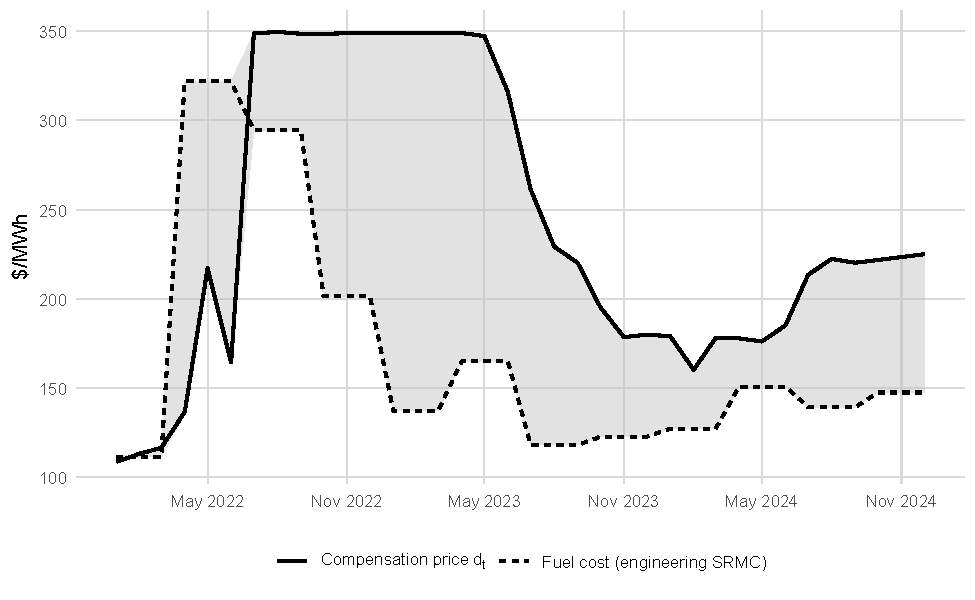
\includegraphics[width=0.9\textwidth]{fig1_compensation_rent}
\caption{The compensation price $\dt$ (trailing-365-day 90th percentile of SA
spot prices) against the focal units' engineering fuel cost, monthly,
2022--2024. The shaded band is the margin between them.}
\label{fig:rent}
\end{figure}

\subsection{The cost of the scheme tracked the lagged price, not the need}

Figure~\ref{fig:costanatomy} shows the quarterly anatomy. Directed volumes
after the synchronous condensers entered service are modest and stable ---
49--77 average megawatts whenever directed, against 117--196 in 2021
(bottom panel) --- and the underlying share of time under direction, the
series validated against AEMO's published statistics in
Section~\ref{sec:data}, peaks in late 2021 and again in late 2023. The recovery cost per directed
megawatt-hour peaks somewhere else entirely: \$416/MWh in 2022Q3, then
\$351--382 from late 2022 through the third quarter of 2023 --- the quarters
when the lagged $\dt$ was paying crisis prices on small volumes. In 2021, three to four times the
directed volume had cost \$85--134 per megawatt-hour. Cost tracked the
formula's memory of last year's prices, not the quantity of security
procured.

\begin{figure}[!htbp]\centering
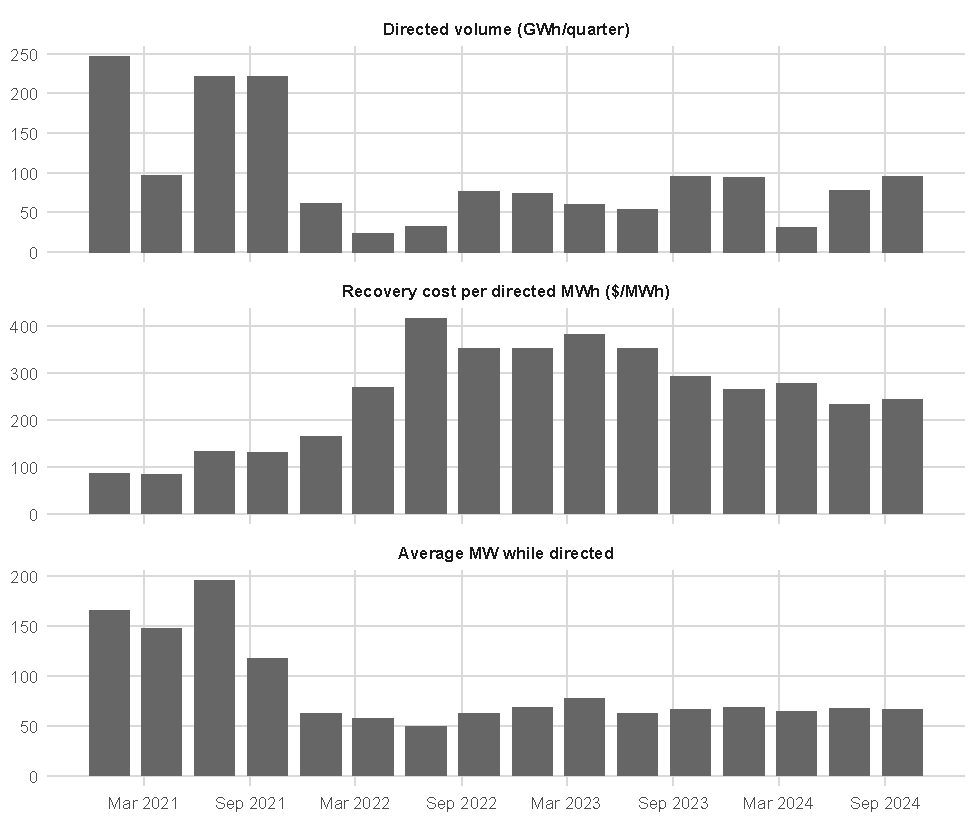
\includegraphics[width=0.9\textwidth]{fig2_direction_cost_anatomy}
\caption{Quarterly directed volume, recovery cost per directed MWh (the NER
3.15.8 recovery amount, AEMO's own cost concept), and average MW online while
directed, 2021--2024.}
\label{fig:costanatomy}
\end{figure}

\subsection{The paid units left the market}

Figure~\ref{fig:supplyhistory} plots, monthly, each station's offered
availability and its cheap tranche (capacity offered at or below \$300/MWh).
Pelican Point behaves like a merchant plant: what it offers, it offers
cheaply, and its availability follows its commercial duty cycle. Torrens
Island B is a different object. Against 600~MW of registered capacity across
the three focal units, the station's offered availability averages well under
200~MW, its cheap tranche under 100~MW; individual units' day-ahead stances declare exactly zero
availability for 47--63\% of all five-minute intervals (in-force bids,
which include within-day revisions and direction periods, show 44--60\%;
Table~\ref{tab:sumstats}), and 2023 --- the peak
of the compensation rent --- is the deepest year of absence, including three
consecutive months (March--May 2023) at literally zero cheap megawatts.
Section~\ref{sec:mechanism} examines what that absence responds to; the
regression sections establish what it correlates with. But the raw scale
deserves stating plainly: through the years in which being directed paid
\$191--272 per megawatt-hour of presence, the direction regime's principal
recipient offered the market as little as the security framework would
tolerate --- and, as Section~\ref{sec:mechanism} shows, never less than
it.\footnote{The roster-versus-requirement comparison finds zero days in 73
opportunities on which the station's declared availability fell short of what
the minimum-combination standard asked of it: absent from the market, the
station remained continuously \emph{directable}.}

\begin{figure}[!htbp]\centering
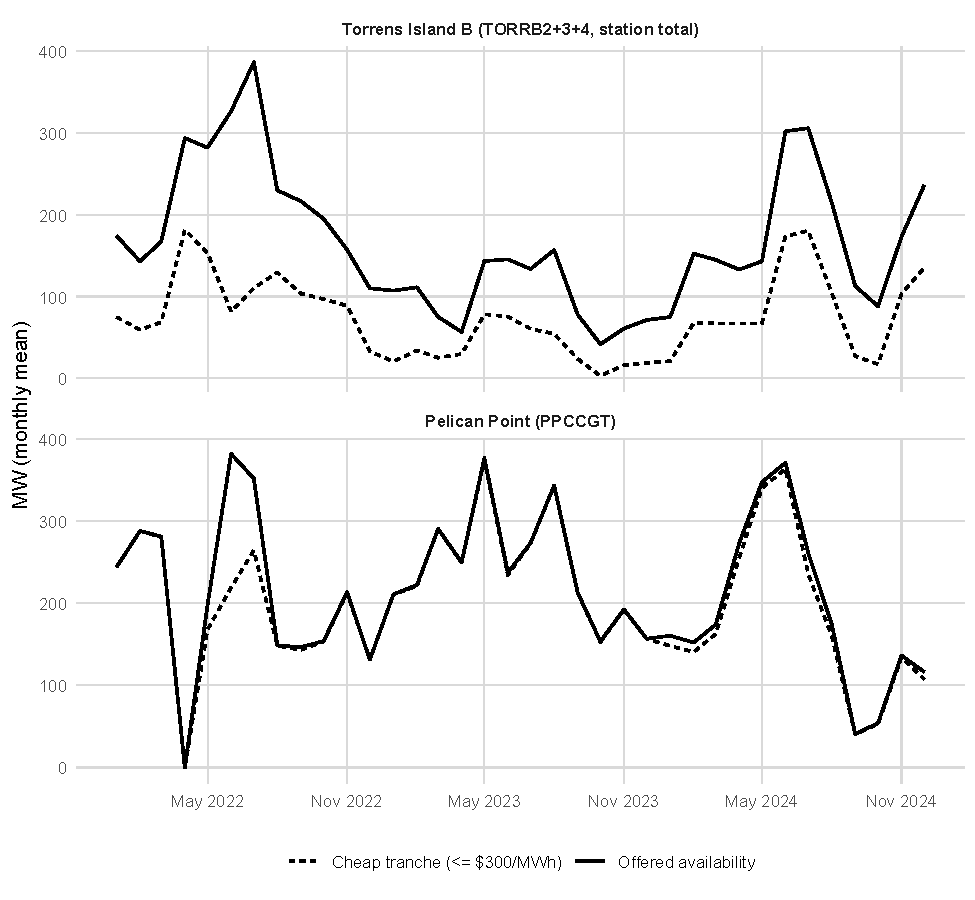
\includegraphics[width=0.9\textwidth]{fig3_supply_history}
\caption{Offered availability and the cheap tranche ($\leq$\$300/MWh),
monthly means, 2022--2024. Torrens Island B is the station total across
TORRB2/3/4 (registered capacity 600~MW).}
\label{fig:supplyhistory}
\end{figure}

% ------------------------------------------------------------------------------
% §5 Empirical design — drafted Phase C from:
%   Direction_clean/README.md (identification logic); 01_outcome findings;
%   stage2_gate_report.md; 03 findings.md (spec, deviations, inference);
%   04 findings.md (matching, power); findings_job2_contamination.md (clean-day rule)
% ------------------------------------------------------------------------------
\section{Empirical Design}\label{sec:design}

\subsection{The outcome: cheap capacity as a share of registered capacity}

The conduct of interest is how much capacity a unit makes available to the
market at prices at which it could actually run. The outcome is the
\emph{cheap-capacity share}: the megawatts a unit offers at or below a cheap
threshold, capped at its declared availability, divided by its registered
capacity. Two co-primary thresholds guard against threshold choice doing the
work: a fixed \$300/MWh, and a cost-indexed $2\times$ the unit's engineering
SRMC that month. The two definitions classify 96--100\% of intervals
identically per unit (worst case 3.9\%, Pelican Point), and a sweep from \$150
to \$500 and from $1.5\times$ to $3\times$ SRMC leaves the Torrens units'
withheld-interval share in an 82--96\% band throughout. Higher values of the
share mean \emph{less} withholding; a negative coefficient on any driver means
more withholding.

The share can fall through two channels with different regulatory treatment:
\emph{capacity withdrawn} (declared availability cut below normal --- physical
withholding) and \emph{capacity priced out} (availability normal, price above
the threshold --- economic withholding). Physical withdrawal dominates for
every unit (51--99\% of withheld intervals, rising to 91\% for Pelican Point),
with a material secondary share (10--33\%) doing both. The Torrens units'
unconditional distribution is bimodal: they sit at the zero-cheap floor in
69--77\% of \emph{all} intervals. Withholding is these units' resting state;
the empirical questions are whether the state deepens when the unit is
essential (RQ1) and whether it tracks the payment for being essential (RQ2).
Appendix~\ref{app:markup} reports the literature's markup lens on the same
offers as a cross-check on this outcome choice.

Three mechanical facts about this market discipline what the share can and
cannot mean, and Section~\ref{sec:results} exploits them directly. First,
the stance is indivisible: dispatch clears the cheapest offered megawatts
first, and a steam unit cannot produce its hundredth megawatt without its
first forty, so there is no bid in which the upper capacity is reachable
while the minimum-stable block is not --- any cheap tranche anywhere on the
ladder self-commits the whole unit. Second, self-commitment is what a
direction pays \emph{against}: compensation covers directed output net of
the counterfactual the unit's own bid establishes, so a unit whose bid
offers nothing has a zero counterfactual and is paid gross, while the same
megawatts offered cheaply would have run at (negative) spot. The one
payoff-relevant object in the bid is therefore binary --- is the
minimum-stable quantum within dispatch's reach, or not --- and the offered
\emph{price} is a dead instrument away from that threshold, which is
exactly how the units treat it (band prices change twice in roughly a
thousand observed bid revisions). Third, the share is accordingly best read
as a posture ruler: its zero point is the order-only stance (the unit runs
only if directed), its distance from zero measures how much running the
unit volunteers, and Section~\ref{sec:results} decomposes it into the
eligibility threshold and the depth beyond it.

\subsection{Essentiality: a rivals-only flag}

A unit-interval is \emph{essential} ($\pex=1$) when no combination of the
\emph{other} available South Australian synchronous units satisfies the minimum
synchronous requirement --- the system needs this unit (for Torrens, the
station) to complete a compliant combination. The flag is built exclusively
from rivals' declared availability; the unit's own bidding and availability
never enter. Two audits confirm the construction. A leakage audit regressing
the flag on the unit's own availability and cheap capacity yields
$R^{2}\in[0.0000, 0.0028]$: the flag is not a repackaging of the unit's own
behaviour. A degeneracy audit confirms essential intervals are non-trivial:
2--6\% of Torrens's and 66\% of Pelican Point's essential intervals still show
the unit bidding as usual, so essential does not mean withheld by
construction.

Essentiality is classified on realised system state rather than the
generator's bid-time forecast. Misclassification relative to the desk's
information set attenuates every essentiality coefficient toward zero; the
estimates below are lower bounds in this specific sense.\footnote{The
direction of the bias follows from the structure of the error, not from
assertion: the flag proxies the desk's expectation, and errors in it are
nondifferential with respect to the outcome conditional on the desk's
information --- realised-state surprises (a rival tripping after bids
closed) are uncorrelated with a bid formed before them. Classical
nondifferential misclassification of a binary regressor biases its
coefficient, and interactions with it, toward zero. What would overturn
this is misclassification correlated with the outcome through a third
channel; the leakage audit ($R^{2}\leq 0.0028$ on the unit's own behaviour)
bounds the obvious candidate.}

\subsection{The competition control: residual-demand slope}

Essentiality bundles two things: eligibility for direction compensation, and
whatever ordinary market power comes with being needed. To separate them, every
specification carries a direct measure of energy-market competition: the slope
of the unit's residual demand curve near the clearing price, built from rivals'
offer stacks net of interconnector imports. More negative slope means rivals
supply more at nearby prices --- more competition; a slope of exactly zero
means rivals are locally saturated --- maximum local market power. The zero
point is a mass point (6.7\% of Torrens intervals), so it enters as a separate
\emph{saturated} indicator alongside the continuous slope.

Two facts about this control, established before any regression, do
substantial interpretive work. First, competition and essentiality are nearly
orthogonal (correlation $-0.036$ for Torrens, $-0.018$ pooled): the control
cannot mechanically absorb the essentiality response. Second, their conditional
relationship runs \emph{opposite} to the market-power story: Torrens's
essential intervals average a residual-demand slope of $-5.04$~MW per \$/MWh
against $-3.31$ in non-essential intervals. Essential periods carry more rival
supply near the clearing price, not less, because essentiality is a
system-security condition that fires in high-renewables, low-demand periods ---
cheap-energy periods --- whereas energy-market scarcity fires elsewhere.
Section~\ref{sec:results} returns to this as the wrong-sign-of-conditions
result.

\subsection{Specifications}

\emph{RQ1.} The essentiality regression, at the unit-interval grain on the
four test units (1,261,576 rows),
\begin{equation}\label{eq:rq1}
\cheap_{it} \;=\; \beta\,\pex_{it} \;+\; \gamma_{1}\,\mathit{slope}_{it}
\;+\; \gamma_{2}\,\mathit{sat}_{it} \;+\; X_{it}'\delta \;+\; \alpha_{i}
\;+\; \mu_{m(t)} \;+\; \varepsilon_{it},
\end{equation}
with unit and month fixed effects and controls $X$ for SRMC, regional demand,
non-synchronous generation, and the spot price.\footnote{The contemporaneous
spot price is itself downstream of conduct and is a bad control in the
strict sense; it is retained because the committed specification included
it. Its own coefficient is indistinguishable from zero in every estimated
model ($p=0.77$--$0.96$ across Table~\ref{tab:rq1}'s specifications), so it
is not doing quiet work.}\footnote{The specification
originally called for the non-synchronous \emph{share} of demand; South
Australian regional demand crosses zero in-sample (rooftop solar), the share
explodes at the crossing, and with the broken control the essentiality
coefficients were inflated roughly tenfold. The level enters instead, with the
share version as a robustness row restricted to demand above 500~MW. The
deviation and its consequences are documented in the analysis record.}
Specification M1 omits the competition terms, M2 adds the slope, M3 adds the
saturated indicator; the movement of $\hat\beta$ from M1 to M3 measures how
much of the essentiality response the energy-market competition channel
absorbs.

\emph{RQ2.} The identifying test. Ordinary market power does not care what
the compensation formula pays; payment-seeking does. On a
coarsened-exact-matched (CEM) sample --- essential unit-intervals matched to
comparison intervals within unit $\times$ month $\times$ non-synchronous
quintile $\times$ hour block $\times$ competition bin cells (140,259 rows;
12,513 essential, a 100\% match rate) --- the regression adds the interaction
of essentiality with the compensation price,
\begin{equation}\label{eq:rq2}
\cheap_{it} \;=\; \theta\,\bigl(\pex_{it}\times \dt/100\bigr) \;+\;
\beta\,\pex_{it} \;+\; \gamma' C_{it} \;+\; X_{it}'\delta \;+\; \alpha_{i}
\;+\; \mu_{m(t)} \;+\; \varepsilon_{it}.
\end{equation}
$\dt$ is monthly, so month effects absorb its level; $\theta$ is identified
from cross-month variation in the essential-versus-matched gap. A negative
$\theta$ --- the gap in the cheap share widening as the payment rises --- is
the payment-seeking signature; a null is the insurance signature, conduct
triggered by the essential state but indifferent to what it pays. This mapping,
including the reading of a null as an informative bound, was written and
committed before estimation.

\emph{June 2022.} The east-coast crisis month contains a market suspension
window and an administered-price period, and holds 19\% of Torrens's essential
unit-rows. Every RQ2 estimate is reported under four treatments: excluding the
suspension window (base), excluding all of June, including the window at the
administered \$300 cap, and excluding pre-suspension June.

\emph{The estimand, stated precisely.} Because $\dt$ is monthly and the
mechanism evidence of Section~\ref{sec:mechanism} shows the posture does not
flex daily, $\theta$ is not a daily behavioural response. It is the
cross-month gradient of a standing posture's \emph{coverage}: how much more
of the essential intervals the order-only stance blankets, relative to
matched intervals, in months when a direction pays more. A policy chosen at
the operating-calendar frequency and tilted --- however it is decided ---
toward the payment environment produces exactly this object, and no claim
about interval-by-interval calibration is made or needed.

\subsection{Inference and hygiene}

Standard errors cluster by month. With 36 clusters (and effectively 21
essential-bearing months in RQ2), analytic clustered inference is supplemented
throughout by a wild cluster bootstrap ($R=999$; Rademacher weights primary,
Webb weights as sensitivity).\footnote{The bootstrap is the unrestricted
variant (\texttt{sandwich::vcovBS}); the null-imposed implementation could not
be installed in the analysis environment. With few effective and unbalanced
clusters the unrestricted variant can be liberal, so the headline estimate
is additionally subjected to randomization inference that imposes the null
by construction (Section~\ref{sec:robustness}), and the null-imposed
bootstrap proper remains a pre-submission upgrade. Analytic and bootstrap
$p$-values agree closely throughout, and every fixed-effects estimate was
re-estimated by explicit-dummy least squares and confirmed numerically
identical.} RQ2's power structure is reported with the
result, not discovered after it: the essential mass spans 21 month-clusters
with 50.8\% of it in the top three, and the compensation price varies across
essential rows with a standard deviation of \$76.6 on a month-level range of
\$121--378.

One design rule, learned from this project's own record and applied to every
day-grain test in Section~\ref{sec:mechanism}: conduct is measured only on
bids formed \emph{outside} direction exposure. On 54\% of essential days the
day-ahead bid was formed while a direction was running or pending, and a bid
formed under direction mechanically shows availability --- treating those days
as choices manufactures state-dependence that evaporates on clean days.
Section~\ref{sec:mechanism} reports the artifact and the correction in full.

% ------------------------------------------------------------------------------
% §6 Results — drafted Phase C from:
%   03_rq1_essentiality/findings.md + findings_3b.md; 04_rq2_compensation_price/findings.md
%   Exhibits: T1, T2, Fig 5
% ------------------------------------------------------------------------------
\section{Results}\label{sec:results}

\subsection{RQ1: essentiality moves conduct for the directed workhorse, and the
competition control absorbs none of it}

Table~\ref{tab:rq1} reports equation~\eqref{eq:rq1}. Pooled across the four
test units, the essentiality coefficient is a precise null on the fixed-\$300
definition ($-0.0045$, wild-cluster-bootstrap $p=0.85$) and negative but
insignificant on the cost-indexed definition ($-0.048$, $p=0.21$). The informative
comparison is across columns: adding the competition controls moves the
essentiality coefficient by 6.2\% and 0.7\% on the two definitions.
Whatever essentiality response exists, the energy-market competition channel
explains essentially none of it.

The pooled numbers average over opposing units. Torrens Island B --- the
station the direction regime actually leans on --- withholds \emph{more} when
essential: $-0.076$ on the cost-indexed definition ($p=0.04$), stable in sign
across all 72 leave-one-month-out re-estimates
(Section~\ref{sec:robustness}). Pelican Point's apparently positive response
($+0.18$) is a one-month artifact --- dropping October 2023 alone flips its
sign --- and is withdrawn as a finding; Table~\ref{tab:rq1} retains it,
footnoted, for completeness.\footnote{The magnitude for Torrens: $-0.076$ of
registered capacity is roughly 15~MW per 200-MW unit, on a station whose
essential-interval cheap offering is already thin.}

Two auxiliary results discipline the interpretation.

\emph{Essentiality is not scarcity.} The competition control itself shows why
the market-power reading of withholding-when-essential fails: essential
intervals are measurably \emph{more} competitive than non-essential ones
(residual-demand slope $-5.04$ versus $-3.31$ for Torrens). An
energy-market-power account of the Torrens response requires essential
periods to be tight;
they are the opposite. The alternative fails on the sign of its conditions,
not merely on magnitude.

\emph{Conduct responds to regimes, not doses.} The one strong conduct
correlate among the controls is the \emph{saturated} indicator: when rivals
are locally saturated, the unit offers 3.2 percentage points less of its
capacity cheaply ($p<0.001$), while the continuous slope carries nothing
($p=0.99$). Conduct moves with the regime of facing no local competition, not
with the degree of competition when some exists. The same shape appears on the
essentiality margin: a response to the essential state. Whether conduct also
scales with what the state \emph{pays} is exactly the RQ2 question, and under
a regime-triggered (insurance) account of withholding the answer should be no.

\subsection{RQ2: the withholding gap widens with the compensation price}

It is not no. Table~\ref{tab:rq2} reports equation~\eqref{eq:rq2}: the
essential $\times$ compensation-price interaction is $-0.051$ per \$100/MWh
on the fixed definition (analytic $p=0.005$; wild-cluster-bootstrap $p=0.004$
Rademacher, $0.004$ Webb) and $-0.055$ on the cost-indexed definition
($p=0.007$; bootstrap $0.007$ and $0.006$). The essential-versus-matched gap in the cheap
share widens by about 5.1 percentage points of registered capacity for every
\$100/MWh of compensation price --- roughly 10~MW per Torrens unit --- and by
about 13 percentage points across the observed \$121--378 range of $\dt$.

\subsection{Decomposing the margin: the response is the eligibility choice}

The share mixes two margins with different economics
(Section~\ref{sec:design}): whether the minimum-stable quantum is within
dispatch's reach at all --- the choice that averts or invites a direction
--- and how much depth is offered when it is. Table~\ref{tab:decomposition}
separates them, with interpretations committed in the project record before
estimation. The dose response lives entirely on the eligibility margin: the
probability that the floor is within reach falls by 8.6 percentage points
per \$100/MWh on essential relative to matched intervals
(wild-cluster-bootstrap $p=0.003$; randomization inference permuting the
month-to-price assignment, $p=0.046$), against a base essential-interval
reach rate of only 10\%. Conditional on the floor being offered, depth shows
no response at all ($p=0.54$--$0.79$). The share coefficient of
Table~\ref{tab:rq2} is this eligibility response diluted by unresponsive
intensive variation --- and the eligibility measure is threshold-free, since
the floor block, when offered, always sits at the $-\$1{,}000$ band. The
same gradient survives aggregation to the month grain
(Figure~\ref{fig:monthgap}): across the 19 essential-bearing months, the
monthly gap moves $-0.096$ per \$100/MWh (HC1 $p=0.001$).

\begin{table}[!htbp]\centering
\caption{Decomposing the dose response: eligibility versus intensive margin}
\label{tab:decomposition}
\begin{adjustbox}{max width=\textwidth}
\begin{threeparttable}
\begin{tabular}{lcc}
\toprule
 & Floor within reach & Offered depth, given reach \\
 & (eligibility margin) & (intensive margin) \\
\midrule
Essential $\times$ compensation price (\$100/MWh) & $-0.086^{***}$ & $0.005$ \\
 & (0.025) & (0.019) \\
Wild-cluster-bootstrap $p$ (Rademacher) & 0.003 & 0.789 \\
Range across June-2022 treatments & $-0.088$ to $-0.076$ & $0.005$ to $0.036$ \\
Randomization-inference $p$ (999 month-permutations) & 0.046 & --- \\
Month-grain WLS slope (19 months, HC1 $p$) & $-0.096$ (0.0012) & --- \\
Observations (base sample) & 140,259 & 28,555 \\
\bottomrule
\end{tabular}
\begin{tablenotes}\footnotesize
\item The eligibility margin is an indicator for the unit's minimum-stable quantum (its frozen floor: 40~MW per Torrens unit) being offered within dispatch's reach; it is identical under both cheap thresholds because the floor block, when offered, sits at the $-\$1{,}000$ band. The intensive margin is the cheap-capacity share on the subsample with the floor in reach (a decomposition aid: it conditions on an outcome). Specification, matching, controls, clustering, and June-2022 treatments exactly as in Table~\ref{tab:rq2}. The cost-indexed intensive margin behaves identically (base $
-0.019
$, $p=
0.55
$). Interpretations for all cells were committed in the project record before estimation.
\item $^{*}p<0.10$, $^{**}p<0.05$, $^{***}p<0.01$ (analytic).
\end{tablenotes}
\end{threeparttable}
\end{adjustbox}
\end{table}


\begin{figure}[!htbp]\centering
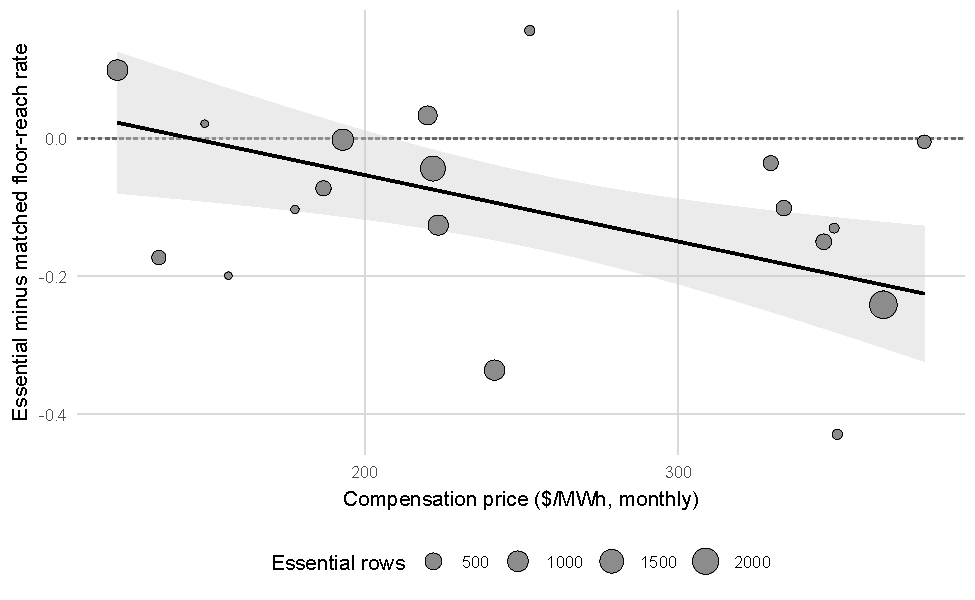
\includegraphics[width=0.85\textwidth]{fig6_month_gap_vs_price}
\caption{The month-grain version of the dose response: the monthly
essential-vs-matched gap in floor-reach against the compensation price,
19 months with at least 30 essential unit-rows, point size proportional to
essential mass. The fitted line is the essential-mass-weighted least-squares
slope ($-0.096$ per \$100/MWh, HC1 $p=0.001$).}
\label{fig:monthgap}
\end{figure}

Unlike the RQ1 level result, the interaction owes nothing to June 2022:
across all four treatments of the crisis month the estimate sits between
$-0.044$ and $-0.058$ with $p$-values of 0.001 to 0.029
(Figure~\ref{fig:rq2stability}). The essential \emph{main effect} in
Table~\ref{tab:rq2} is positive ($+0.089$): at low compensation prices,
essential intervals show \emph{more} cheap capacity than matched ones ---
these are winter-tight periods in which running pays --- and the gap
crosses zero at $\dt\approx\$175$, visible directly in the month-grain
scatter (Figure~\ref{fig:monthgap}). The dose response is not a deepening
of an always-negative gap; it is a reversal, from relative presence when
the direction channel pays little to relative absence as it pays more. Attenuation from realised-state
classification biases $\theta$ toward zero, so the true payment-sensitivity is
if anything larger.

The channel ranking, under the interpretation committed before estimation,
is then: energy-market power --- eliminated on the wrong sign of its
conditions; pure presence-inelasticity with no payment sensitivity --- the
insurance account of Section~\ref{sec:design} --- rejected, because it
predicted a null here; payment-seeking --- the account most consistent with
the data. One refinement of the regime-not-dose pattern survives
alongside: conduct is regime-triggered on the \emph{competition} margin
(saturation, not slope), while on the \emph{payment} margin the essential-state
response scales with the prize.

Two limitations are reported with the estimate, as committed with the
design before estimation. The interaction is identified from cross-month
variation; anything that widens the essential-versus-matched gap \emph{and}
co-moves with the compensation price across months --- 2022H2 fuel-supply
stress is the obvious candidate --- is not excluded by month effects.
Section~\ref{sec:robustness} confronts this directly with the timing wedge
the formula creates (gas fell nine months before the payment did) and a
fuel horse race; the pure fuel story fails its point predictions there, but
the sharpest formula-driven contrast is marginal, so this paper's causal
language for the cross-month gradient is deliberately ``consistent with
payment-seeking,'' not proof. And the essential mass is concentrated: 21
effective month-clusters, half the mass in three of them. The estimate
clears conventional significance under bootstrap inference designed for
this cluster structure and under randomization inference
(Table~\ref{tab:decomposition}), but the concentration stands as a stated
limitation.

A third limitation deserves its own statement: the treatment is not
mechanically exogenous to the units that receive it. The compensation price
is a percentile of past regional spot prices, and withholding that raises
spot prices feeds, with a lag, the units' own future payment. Three facts
bound the loop without eliminating it. Contemporaneously it is negligible
by construction --- a month's own conduct enters its own $\dt$ only through
that month's marginal contribution to a 365-day window. Dynamically, the
loop requires the units' absence to move the \emph{top-decile} prices that
set the percentile, and the record places their absence where prices are
low: essential intervals are the market's more-competitive, cheap-energy
periods (Section~\ref{sec:results}), not its price spikes. And the one
large movement in $\dt$ over the sample --- the 2022 surge to \$349 ---
tracked NEM-wide fuel costs (\$322/MWh at the focal units' own heat rates),
a system event no three units authored. What survives as a caveat is the
softer form: any residual own-price influence inflates the payment
gradient's causal reading, and the paper's ``consistent with'' language is
calibrated to that residual as well.

\begin{table}[!htbp]\centering
\caption{RQ1: Essentiality and the cheap-capacity share}
\label{tab:rq1}
\begin{adjustbox}{max width=\textwidth}
\begin{threeparttable}
\begin{tabular}{lcccccc}
\toprule
 & \multicolumn{2}{c}{M1} & \multicolumn{2}{c}{M2} & \multicolumn{2}{c}{M3} \\
\cmidrule(lr){2-3}\cmidrule(lr){4-5}\cmidrule(lr){6-7}
 & Fixed \$300 & 2$\times$SRMC & Fixed \$300 & 2$\times$SRMC & Fixed \$300 & 2$\times$SRMC \\
\midrule
\multicolumn{7}{l}{\emph{Panel A: pooled (four focal units)}} \\
Essential & $-0.004$ & $-0.048$ & $-0.004$ & $-0.048$ & $-0.004$ & $-0.048$ \\
 & (0.023) & (0.038) & (0.023) & (0.038) & (0.023) & (0.038) \\
 & [0.847] & [0.208] & [0.847] & [0.207] & [0.857] & [0.207] \\
Saturated (slope $=0$) & & & & & $-0.032^{***}$ & $-0.036^{***}$ \\
 & & & & & (0.006) & (0.007) \\
\midrule
\multicolumn{7}{l}{\emph{Panel B: heterogeneity (M3 specification)}} \\
Essential, Torrens Island B only & & & & & $-0.037$ & $-0.076^{**}$ \\
 & & & & & (0.023) & (0.036) \\
Essential, Pelican Point only\tnote{a} & & & & & $0.184^{*}$ & $0.128$ \\
 & & & & & (0.099) & (0.084) \\
\midrule
Observations (pooled) & \multicolumn{6}{c}{1,261,576} \\
\bottomrule
\end{tabular}
\begin{tablenotes}\footnotesize
\item Outcome: share of registered capacity offered below the cheap threshold (fixed \$300/MWh or 2$\times$ engineering SRMC), 5-minute unit--interval panel, 2022--2024. M1 adds demand, non-synchronous supply, SRMC, and price controls; M2 adds the residual-demand slope; M3 adds the saturated (zero-slope) indicator. Analytic standard errors clustered by month in parentheses; wild cluster bootstrap $p$-values (Rademacher, $R=999$, 35 df) in brackets for the essentiality coefficient. Panel B re-estimates M3 on the Torrens Island B and Pelican Point subsamples.
\item[a] The Pelican Point coefficient is not robust: it flips sign when October 2023 is dropped (leave-one-month-out, Section~\ref{sec:robustness}) and is withdrawn as a finding.
\item $^{*}p<0.10$, $^{**}p<0.05$, $^{***}p<0.01$ (analytic).
\end{tablenotes}
\end{threeparttable}
\end{adjustbox}
\end{table}

\begin{table}[!htbp]\centering
\caption{RQ2: The essential-interval withholding gap widens with the compensation price}
\label{tab:rq2}
\begin{adjustbox}{max width=\textwidth}
\begin{threeparttable}
\begin{tabular}{lccc}
\toprule
 & \multicolumn{2}{c}{Essential $\times$ compensation price (\$100/MWh)} & \\
\cmidrule(lr){2-3}
Sample treatment of June 2022 & Fixed \$300 & 2$\times$SRMC & $N$ \\
\midrule
Base (exclude June-2022 suspension window) & $-0.051^{***}$ & $-0.055^{***}$ & 140,259 \\
 & (0.016) & (0.019) & \\
(i) Exclude all June 2022 & $-0.051^{***}$ & $-0.058^{***}$ & 134,636 \\
 & (0.016) & (0.016) & \\
(ii) Include window at APC \$300 & $-0.044^{**}$ & $-0.050^{**}$ & 144,358 \\
 & (0.019) & (0.020) & \\
(iii) Base minus pre-suspension June & $-0.051^{***}$ & $-0.058^{***}$ & 135,269 \\
 & (0.016) & (0.016) & \\
\midrule
Essential (main effect, base sample) & $0.089^{*}$ & $0.083$ & \\
 & (0.049) & (0.058) & \\
\midrule
WCB $p$ (base row): Rademacher & 0.004 & 0.007 & \\
\phantom{WCB $p$ (base row):} Webb & 0.004 & 0.006 & \\
\bottomrule
\end{tabular}
\begin{tablenotes}\footnotesize
\item Coefficient on essential $\times$ compensation price (per \$100/MWh) on the CEM-matched sample (unit $\times$ month $\times$ non-synchronous quintile $\times$ hour block $\times$ competition bin). A coefficient of $-0.051$ means the essential-vs-matched gap in the cheap-capacity share widens by 5.1 percentage points of registered capacity per \$100/MWh. Analytic standard errors clustered by month in parentheses; specification and controls as in Table~\ref{tab:rq1} (M3). Wild cluster bootstrap $p$-values ($R=999$, 20 df) for the base sample. The interpretation of this test, including the reading of a null, was committed in the project record before estimation.
\item $^{*}p<0.10$, $^{**}p<0.05$, $^{***}p<0.01$ (analytic).
\end{tablenotes}
\end{threeparttable}
\end{adjustbox}
\end{table}


\begin{figure}[!htbp]\centering
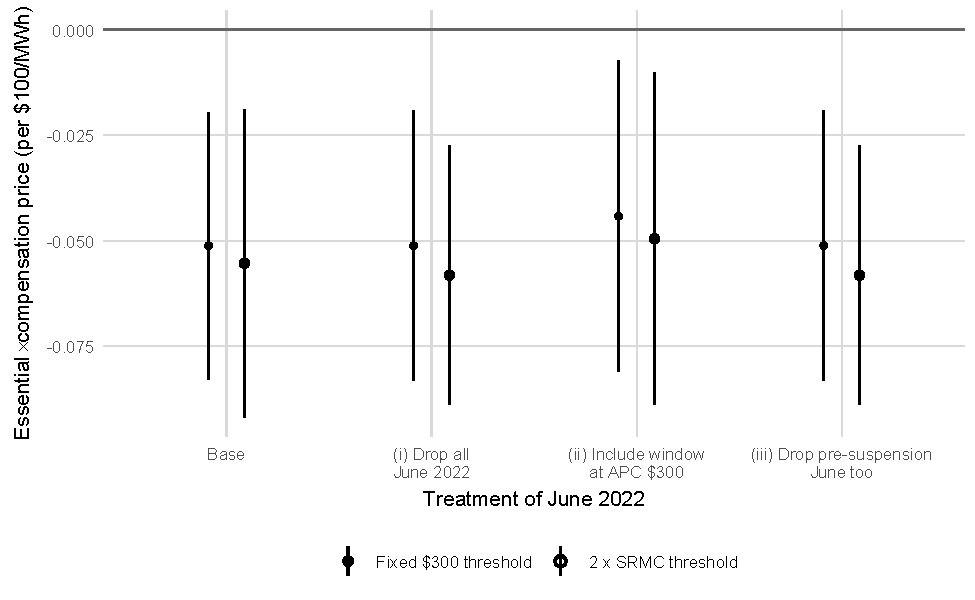
\includegraphics[width=0.85\textwidth]{fig5_rq2_stability}
\caption{The RQ2 interaction across June-2022 treatments and outcome
definitions. Points are estimates of $\theta$ in
equation~\eqref{eq:rq2}; bars are 95\% analytic confidence intervals,
clustered by month. All eight estimates lie between $-0.044$ and $-0.058$ per
\$100/MWh.}
\label{fig:rq2stability}
\end{figure}

% ------------------------------------------------------------------------------
% §7 Mechanism — drafted Phase C from:
%   interpretation_staged_framework.md (+ amendments); findings_job2_contamination.md;
%   findings_task1.md / task1b.md (post-fix); findings_task5b.md; findings_task9/10;
%   Exhibits: T3
% ------------------------------------------------------------------------------
\section{Mechanism: A Standing Posture, Not a Daily Calibration}\label{sec:mechanism}

The regression results say that withholding deepens with the compensation
price where the scheme's eligibility bites. This section opens the conduct up
at the level of individual bids, days, and direction episodes. The picture
that emerges is specific: the absence is a \emph{standing posture} --- chosen
at the day-block level, indifferent to the daily security envelope and to the
daily prize --- and the compensation mechanism pays gross rates into that
posture whenever the system's need makes the unit essential. The section ends
with the two findings that discipline any stronger claim: a state-dependence
result this project itself withdrew after a contamination audit, and the
grain at which the dose response does and does not appear.

\subsection{What a direction buys, and what it pays}

Across the 740 direction episodes with a resolved in-force bid, directed
output equals the unit's operating floor almost exactly: median directed
output 40~MW per Torrens unit --- the floor block itself --- with 55.9\% of
episodes delivering zero or negative excess over the floor and 80.8\% within
25~MW (Figure~\ref{fig:floor}). A direction buys presence, not energy.

It pays as if it bought energy at scarcity prices. Compensation reconciles to
$0.95 \times \text{directed MWh} \times \dt$ with $R^{2}=0.99$
(Section~\ref{sec:setting}), and the aggregate consequence over 2022--2024 is
the mechanism's headline economics: the direction channel paid the three
Torrens units \$141.9M for 625,635 directed MWh --- their 683 episodes of
the 740 above --- that would have earned \$7.2M
at spot prices over the same windows --- a \$134.7M gap, a ratio of roughly
20 to 1 that holds for every unit in every year. In 2023 the market value of the directed output
was \emph{negative} for all three units: 48.2\% of directed megawatt-hours
were delivered into negative spot prices. Nor is the comparison distorted by
averaging: at the interval level, spot exceeds marginal fuel cost in 3.9\% of
directed intervals, the median directed interval loses \$141/MWh at fuel cost
alone, and only 11 of 683 episodes (1.6\%) were profitable on average. There
is no commercial running inside these windows to forgo. Given these relative
payment rates, a standing absent posture is not a puzzle to be explained ---
it is the only stance an informed desk would hold.

\subsection{The posture is standing, not state-dependent}

Three tests --- each with its interpretation committed in the project
record before estimation --- all on bids formed outside direction exposure
(the clean-day rule of Section~\ref{sec:design}), locate the choice; the
broader $N-1$ essentiality flag they require is constructed and validated in
Appendix~\ref{app:n1}.

\emph{The base rate.} The units' day-ahead bids withhold or price out the
floor megawatts on 76--80\% of all clean days --- essential or not. Absence is
the resting state, held in multi-day blocks (median unavailability spell 2--4
days, maxima up to 100 days), total rather than partial (when the units withdraw
they declare zero, not a derating: sub-floor positive declarations are 0.2\%
of intervals), and organised as a rotating one-to-two-of-three station roster
(all three Torrens units are on offer together on 4\% of days, and unit
availabilities are deliberately anti-correlated).

\emph{The exit act is event-timed, not need-timed.} On clean days when a
Torrens unit has an evening on offer, cancelling it is \emph{less} likely ---
by 16 percentage points off a 22.5\% base ($p=0.02$, bootstrap $p=0.017$;
Table~\ref{tab:mechanism}, column 1) --- when the system is one contingency
from needing the unit. A loss-timing account fails alongside: cancellations
are less likely, not more, when the previous day's prices imply running
losses (column 2, wrong sign at $p=0.005$). The evening exits that precede
directions sit in the direction run-up itself, not in the security calendar
or the loss calendar.

\emph{The price of presence does not move either.} When the units offer their
floor megawatts at all, they offer them at the floor-band price ---
essentially $-\$1{,}000$ --- in essential hours, in ordinary hours, and on
ordinary days alike: the essential-day effect on the offered floor price is
+\$45 ($p=0.86$; column 4), and Pelican Point's within-day essential-hour
effect is exactly zero. The pricing margin
joins the availability margin: the posture is set by the day-block and does
not respond to the envelope.

\begin{table}[!htbp]\centering
\caption{Mechanism: the exit act is state-dependent; floor pricing is not}
\label{tab:mechanism}
\begin{adjustbox}{max width=\textwidth}
\begin{threeparttable}
\begin{tabular}{lcccc}
\toprule
 & \multicolumn{3}{c}{Exit act (evening offered share)} & Floor price (\$/MWh) \\
\cmidrule(lr){2-4}\cmidrule(lr){5-5}
 & (1) & (2) & (3) & (4) \\
\midrule
Essential ($N{-}1$) & $-0.162^{**}$ & $-0.124^{*}$ & & $45.3$ \\
 & (0.066) & (0.065) & & (265.3) \\
Essential ($N{-}1$) $\times$ expected loss & & $-0.001^{***}$ & & \\
 & & (0.000) & & \\
$N{-}1$ only (not $N{-}0$) & & & $-0.190^{***}$ & \\
 & & & (0.061) & \\
Directly pivotal ($N{-}0$, \textit{pex}) & & & $-0.001$ & \\
 & & & (0.106) & \\
\midrule
Observations & 473 & 473 & 473 & 650 \\
\bottomrule
\end{tabular}
\begin{tablenotes}\footnotesize
\item Day-level regressions on clean days (bids formed outside direction exposure), $N{-}1$ essentiality flag (Task~7 construction). Columns (1)--(3): outcome is the evening offered share (exit act); column (2) adds the expected foregone-loss control and its interaction; column (3) splits essentiality into tiers. Column (4): outcome is the offered floor price. Wild-cluster-bootstrap-based inference in the source analysis confirms column (1) at $p=0.017$. Standard errors clustered by month in parentheses. Both tests' interpretations were committed in the project record before estimation; the $N{-}1$ flag construction is Appendix~\ref{app:n1}.
\item $^{*}p<0.10$, $^{**}p<0.05$, $^{***}p<0.01$ (analytic).
\end{tablenotes}
\end{threeparttable}
\end{adjustbox}
\end{table}


\begin{figure}[!htbp]\centering
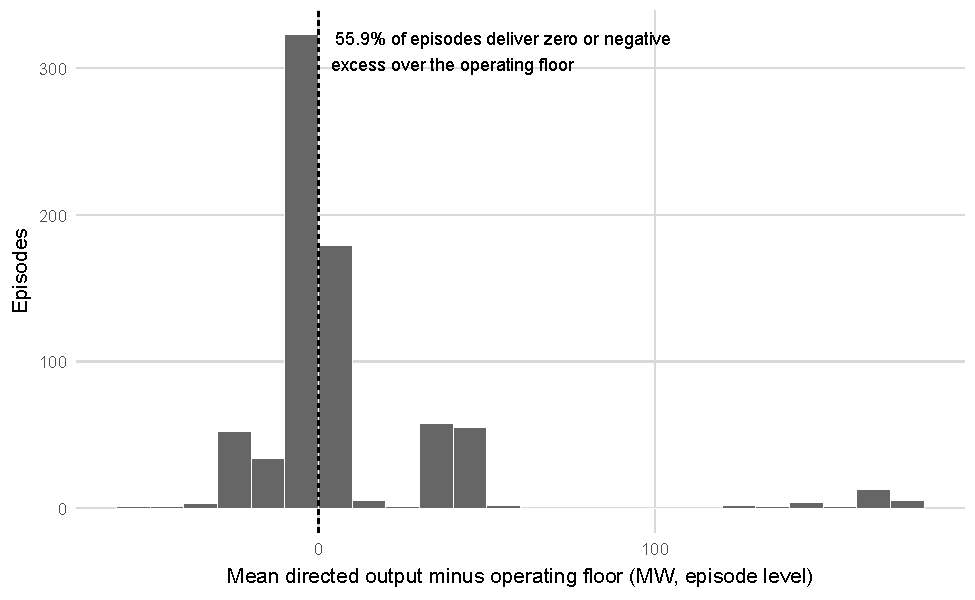
\includegraphics[width=0.8\textwidth]{fig4_output_vs_floor}
\caption{Directed output relative to the unit's operating floor, for the 740
direction episodes with a resolved in-force bid, 2022--2024. The mass at zero
is the institutional design: a direction compels presence at minimum stable
load.}
\label{fig:floor}
\end{figure}

\subsection{A withdrawn result: the contamination audit}

An earlier day-grain version of the essentiality test in this project found
what looked like clean state-dependence: units withdrew 12.7 percentage
points more on essential days ($p<0.001$). The finding did not survive its
own audit, and the correction is reported here as part of the result. On 54\%
of essential days, the day-ahead bid was formed while a direction was running
or pending; a bid formed under direction mechanically shows availability. On
the 80 essential days with cleanly formed bids the withdrawal effect is
$-0.015$ ($p=0.71$): the apparent state-dependence was the direction itself
sitting in the measured bids. What survives on the clean record is the
standing posture --- and the fact that 95.4\% of the 280 clean-day first
directions arrived at a day-ahead stance that had already withdrawn (71.8\%)
or priced out (23.6\%) the floor megawatts. The system directs into a posture
that predates its need.

\subsection{Reconciling the grains}

The clean-day, day-grain dose-response test is null (49 essential days over
14 months; all interactions $p=0.50$--$0.96$), while the interval-grain
matched test of Section~\ref{sec:results} finds $-0.051$ per \$100/MWh at
$p<0.01$. These are not in tension; they are different instruments pointed at
the same object. The day-grain test conditions on clean essential days ---
which the contamination audit shows are scarce precisely because the
direction regime blankets essential periods --- and its wide confidence
intervals cannot exclude effects several times the interval estimate. The
interval-grain test pools 12,513 essential unit-intervals against matched
comparisons with 300 times the observations. The honest summary is a powered
estimate and an uninformative bound, not a conflict. What the day-grain
record does add is the shape of the response: the posture does not flex
day-to-day with the envelope or the prize (this section), while its depth
across months tracks what essentiality pays (Section~\ref{sec:results}).
Both are what a policy chosen once --- and paid gross whenever the system's
need arrives --- would produce.\footnote{The daily activity around the
standing choice is stage-appropriate housekeeping, not repositioning:
document-revision activity ramps into directions (a vigilance signature), but
net availability and price-ladder movement around direction issue is
approximately zero. A desk that watches the weather and a desk that watches
the direction calendar are watching the same clock in this system; the staged
pattern shows the desk is informed, and this paper deliberately does not use
it to establish motive. The economic content is in the mechanism's design, not in generator
sophistication.}

% ------------------------------------------------------------------------------
% §8 Robustness — drafted Phase C from:
%   findings_3b.md (LOMO, June split); 03 findings (deviations, share row);
%   04 findings (treatments); 01 findings (thresholds, audits); rq1_wcb.csv
% ------------------------------------------------------------------------------
\section{Robustness}\label{sec:robustness}

\subsection{Leave-one-month-out}

Both headline unit-level RQ1 results were re-estimated 72 times, dropping one
month at a time under both outcome definitions. The Torrens coefficient is
negative in all 72 re-estimates; every flagged month is a $p$-value crossing
in the 0.03--0.15 band, never a sign change. Pelican Point fails the same
diagnostic: dropping October 2023 alone flips its sign (from $+0.184$ to
$-0.083$ fixed; $+0.128$ to $-0.105$ cost-indexed), and dropping two other
months moves it across the 5\% threshold in the opposite direction. The
asymmetry is the basis for the treatment in Section~\ref{sec:results}: Torrens
is a stable borderline-significant response; Pelican Point's positive
coefficient is a one-month artifact and is withdrawn.

\subsection{June 2022}

The crisis month is handled segment-by-segment using AEMO's own per-interval
flags (suspension window 15--24 June; administered pricing from 5 June). For
the RQ1 Torrens result: dropping the suspension window alone leaves the
coefficient intact ($-0.068$, $p=0.054$ cost-indexed), as does dropping the
pre-suspension fortnight alone ($-0.058$, $p=0.045$); only removing all of
June --- 19\% of Torrens's essential unit-rows, with zero essential rows after
the suspension --- degrades it to $p=0.13$. The dependence is on June's
essential-interval mass, a statistical-power statement, not on
suspension-era administered pricing, a confounding story. The RQ2 interaction
needs no such parsing: all four June treatments give $-0.044$ to $-0.058$
($p=0.001$--$0.029$; Figure~\ref{fig:rq2stability}).

\subsection{The timing wedge: separating the payment from the fuel}

The formula's memory creates a test the referee's fuel-confound story must
pass: gas prices fell in October 2022, but the trailing-percentile $\dt$
kept paying crisis rates until July 2023. If the essential-versus-matched
gap were fuel-stress conduct wearing the payment's clothes, it should have
collapsed with gas, nine months before the payment fell. It did not. With
the sample split at the calendar boundaries fixed in advance --- early 2022
($\dt\approx\$176$, a placebo-in-time), the crisis quarter (gas and $\dt$
both high), the lag-wedge (gas low, $\dt\approx\$340$), and the
post-roll-off period (both low, omitted) --- the eligibility-margin gap is
$-0.100$ in the crisis quarter ($p=0.03$), $-0.075$ through the lag-wedge
(bootstrap $p=0.089$), statistically indistinguishable from the crisis
value, and zero in both low-payment regimes despite their opposite fuel
conditions. The four period gaps order monotonically with the payment, not
with gas. What keeps this supportive rather than decisive is power: the
lag-wedge holds four essential-bearing months, and its contrast clears only
the 10\% level --- hence the ``consistent with'' language maintained
throughout this paper.

A conditional horse race points the same way within its limits. Adding
essential $\times$ gas alongside essential $\times$ $\dt$ (series
correlated at 0.48 across months), the payment interaction retains its full
magnitude and significance on the cheap-share outcome ($-0.054$, $p=0.013$)
with the gas interaction at exactly zero ($p=0.85$); on the eligibility
margin the two collinear series split the variance and neither is
individually significant --- a limitation of conditioning, which is why the
timing design above, not the horse race, carries the identification weight.

A placebo unit --- often essential but outside the compensation channel ---
does not exist in this market, for a reason that is itself informative:
essentiality concentrates on precisely the units the direction channel
pays. The candidate stations with constructed essentiality flags
(Quarantine, Dry Creek, Mintaro, Barker Inlet, Snapper Point) have 0--45
essential intervals in three years against Torrens's 4,083, and most are
themselves directed. The treatment set and the missing placebo have the
same cause.

\subsection{Inference and measurement}

Webb-weight bootstrap $p$-values match Rademacher throughout (RQ2 base case:
0.0040 versus 0.0041 fixed; 0.0061 versus 0.0073 cost-indexed). Because the
unrestricted wild bootstrap can be liberal with few unbalanced clusters,
the eligibility-margin estimate was additionally subjected to randomization
inference that imposes the null by construction --- permuting the
month-to-price assignment across the 36 sample months, 999 draws --- giving
$p=0.046$ (Table~\ref{tab:decomposition}); the null-imposed bootstrap
proper requires a compilation toolchain unavailable in the analysis
environment and remains a pre-submission upgrade. The two
outcome definitions agree on 96--100\% of interval classifications and on
every substantive conclusion. Threshold sweeps (\$150--\$500 fixed;
$1.5\times$--$3\times$ SRMC) leave the Torrens classification in an 82--96\%
band. The non-synchronous share specification (restricted to demand above
500~MW, avoiding the zero-crossing) gives $-0.017$/$-0.064$ for the pooled
essentiality coefficient --- same sign, same conclusion as the level
specification. The essentiality flag survives its leakage audit
($R^{2}\leq 0.0028$ on the unit's own behaviour) and its degeneracy audit
(essential intervals include units bidding as usual).

\subsection{An earlier design, reported not buried}

Before the matched interval design of Section~\ref{sec:design}, this project
ran a coarser opportunity-set version of the same question: does a withheld
indicator interact with $\dt$ on intervals where withholding could plausibly
cause a direction? That design is null (pooled interaction $t=1.55$,
$p=0.14$; one unit marginal at $p=0.07$), and Appendix~\ref{app:withhold_opportunity}
reports it in full. Two reasons it is superseded rather than averaged in: the
binary withheld outcome discards the intensive margin where
Section~\ref{sec:results}'s effect lives, and its opportunity flag conditions
on system state less sharply than the CEM match. The null is consistent with
the pattern in Section~\ref{sec:mechanism} --- the extensive-margin posture
does not flex with the prize; its depth does.

% ------------------------------------------------------------------------------
% §9 Discussion & policy — drafted Phase C from:
%   findings_task5b.md; findings_task11 (era split, lag-wedge); findings_task13;
%   plan §9; memory: project_sa_regime_exit_2025
% ------------------------------------------------------------------------------
\section{Discussion and Policy Implications}\label{sec:discussion}

\subsection{The conduct is a property of the design}

The mechanism that generates this paper's findings can be stated in one
sentence: South Australia's direction scheme paid gross output at a
backward-looking scarcity price to units whose market alternative was running
at a loss. Each clause contributes. \emph{Gross} payment severs compensation
from the counterfactual, so a unit whose bids establish a low counterfactual
loses nothing by establishing it. The \emph{backward-looking} reference price
held the margin over fuel cost above \$100/MWh for eleven consecutive months
after the 2022 crisis --- peaking at \$211/MWh --- by formula. And the \emph{loss-making market alternative} --- spot
above fuel cost in 3.9\% of directed intervals --- removes any opportunity
cost of absence. Under these payoffs, a standing withdrawn posture dominates
commitment across essentially all conditions, which is exactly the shape of
conduct the mechanism sections document: absence as the resting state,
indifferent to the daily envelope and the daily prize, with depth across
months that tracks what essentiality pays.

The distinction between a standing posture and daily optimisation matters for
how the conduct should be judged. Nothing in this record shows a desk
manipulating the system's need day by day; the informative daily signals ---
event-timed exits, unmoved floor prices, a roster that never falls below the
security standard's ask --- are consistent with a fixed policy plus
housekeeping. The policy itself, however, is priced: the dose response of
Section~\ref{sec:results} is the signature of conduct that sorts on the
payment, and the \$134.7M gap between what the direction channel paid and
what the same megawatt-hours were worth is the transfer that policy earned.
A regulator does not need to prove daily intent to conclude that the scheme
bought its own necessity.

Two scope statements keep the accounting honest. First, the 20-to-1 figure
compares \emph{payment rates on the same megawatt-hours}, not welfare: the
scheme was buying system security, which the spot price of energy does not
value, and the right normative benchmark is the cost of the cheapest
alternative supply of the same service --- the synchronous condensers whose
entry collapsed intervention costs are the revealed measure, and the
counterfactual in which unprofitable units simply retire rather than wait
for directions would have forced that comparison earlier. What the transfer
figure establishes is not a welfare loss of that size but the price
pressure the design placed on a service procurable otherwise. Second, an
owner-level motive this paper cannot fully separate is the gentailer
portfolio: the units' owner retails electricity, and withholding that
raises spot prices pays a portfolio even when it loses the plant money. The
wrong-sign result disciplines this too --- portfolio market power wants
absence in scarce, high-price hours, and the essential intervals where the
absence concentrates are measurably the opposite --- but as a residual
account of the level of withholding (rather than its payment gradient) it
is acknowledged, not excluded.

\subsection{Design alternatives}

Each defect maps to a repair, and the repairs are standard tools of the
capacity-remuneration literature \citep{CramtonOckenfelsStoft2013_capacity,
Fabra2018_capacity}.

\emph{Pay the wedge, not the gross.} Compensating the increment over a
counterfactual dispatch --- or, equivalently, netting retained market revenue
against costs actually incurred --- restores the opportunity-cost margin that
gross payment deletes. The objection that counterfactuals are gameable is
real but misdirected here: the current design already depends on a
counterfactual, the unit's own bid, and pays as if it were zero. The American
reliability-must-run experience documented the same class of defect two
decades earlier: contract forms whose payments were disconnected from market
outcomes created serious incentive problems and raised prices, prompting
redesign \citep{BushnellWolak1999_rmr, BushnellWolak1999_leverage}.

\emph{Look forward, not back.} A trailing-percentile reference price imports
last year's scarcity into this year's payment. Any forward-looking or
cost-anchored reference --- a fuel-indexed price, as this paper's cost-indexed
outcome definition already constructs, or a periodically reset administered
price --- would have cut the 2023 payments roughly in half without touching
the scheme's security function.

\emph{Procure presence explicitly.} The deepest fix prices the actual
commodity. What the system bought was synchronous presence: a known number of
machine-hours per day, from a known set of units. A contracted availability
product converts the rent into a competitive tender and removes the incentive
to be absent at all; the synchronous condensers that ended the bulk direction
era in 2021 (Section~\ref{sec:setting}) are the network-side version of the
same principle --- buy the service, not the emergency.

\subsection{Epilogue: the regime exits}

In September 2025 the minimum synchronous requirement fell to one unit, with
zero targeted once Project EnergyConnect's second stage completes. The
direction channel that paid \$141.9M to three units over 2022--2024 is
closing, not because the conduct was policed but because the underlying
scarcity --- synchronous strength in a renewables-dominated grid --- was
engineered away by transmission and synchronous condensers. That is the final
sense in which the economics of this episode live in the mechanism's design:
the payments were a bridge between an old fleet and a grid that no longer
needs it, and the bridge's toll was set, for three years, by a formula
looking the wrong way.


\clearpage
\bibliography{../Bibliography_base}

\clearpage
\appendix
% ------------------------------------------------------------------------------
% Appendix A — drafted Phase C from Direction/outputs/withhold_opportunity/
%   stage2/3/4/4b findings; Exhibit: T4
% ------------------------------------------------------------------------------
\section{An Earlier Opportunity-Set Design}\label{app:withhold_opportunity}

Before the matched interval design of Section~\ref{sec:design}, the
project's first, registered-in-advance pass at the payment-sensitivity question used
an opportunity-set construction: flag intervals in which the unit's withholding
could plausibly cause a direction (rivals near the security boundary), match
them to comparison intervals by coarsened exact matching on system state, and
test whether a binary withheld indicator interacts with the compensation
price,
\[
\mathit{withheld}_{it} = \lambda\,(\dt \times \mathit{opp}_{it}) +
\phi\,\mathit{opp}_{it} + \kappa\,\mathit{srmc}_{it} + \alpha_i +
\eta_{q(it)} + \omega_{h(it)} + \varepsilon_{it},
\]
with unit, non-synchronous-quintile, and hour-block fixed effects, clustered
by month.

Table~\ref{tab:withhold_opp} reports the result: null. The pooled interaction
is $0.00024$ ($t=1.55$, $p=0.14$), with only TORRB4 marginal ($p=0.07$) and
the sister units on either side of zero. The June-2022 gap in the
compensation-price series, 19\% of opportunity intervals, is handled by
imputation at \$164.38/MWh as a robustness variant with the same conclusion.
A sign-flip diagnostic confirms TORRB3's wrong-signed estimate is
within-sample noise, not composition: the three Torrens units' opportunity
sets are byte-identical (the essentiality state is a station-level object),
so cross-unit differences on identical regressor sets are sampling variation.
Pelican Point's cell is uninformative --- its opportunity intervals fall in a
narrow calendar window with essentially no $\dt$ variation.

Two design features explain why this test is superseded rather than pooled
with Section~\ref{sec:results}. First, the outcome is a binary withheld
indicator, and Torrens's withheld rate inside the matched strata is already
high on both sides of the contrast (90--94\% in comparison intervals,
97--99\% in opportunity intervals): the extensive margin is nearly saturated,
so the test can only detect movement in a thin residual band. The interval design's
continuous cheap-capacity share carries the intensive margin where the
estimated response lives. Second, the opportunity flag conditions on rivals'
proximity to the boundary more coarsely than the CEM competition bins.
The null is nonetheless informative, and consistent with the mechanism
picture: on the extensive margin the posture does not flex with the prize.

\begin{table}[!htbp]\centering
\caption{Appendix: earlier opportunity-set design --- $d_t \times$ opportunity interaction (withheld indicator)}
\label{tab:withhold_opp}
\begin{adjustbox}{max width=\textwidth}
\begin{threeparttable}
\begin{tabular}{lccc}
\toprule
 & $d_t \times$ opp & $d_t^{robust} \times$ opp & $N$ \\
\midrule
Pooled & $0.00024$ & $0.00019$ & 177,854 \\
 & (0.00016) & (0.00013) & \\
TORRB2 & $0.00021$ & $0.00030$ & 57,677 \\
 & (0.00027) & (0.00021) & \\
TORRB3 & $-0.00018$ & $-0.00013$ & 57,677 \\
 & (0.00027) & (0.00024) & \\
TORRB4 & $0.00055^{*}$ & $0.00034$ & 57,677 \\
 & (0.00029) & (0.00026) & \\
PPCCGT\tnote{a} & $0.00061$ & $-0.00125$ & 4,823 \\
 & (0.00129) & (0.00400) & \\
\bottomrule
\end{tabular}
\begin{tablenotes}\footnotesize
\item Linear probability model: withheld $\sim d_t \times$ opportunity $+$ SRMC with unit, non-synchronous-quintile, and hour-block fixed effects on the CEM-matched sample, clustered by month. $d_t^{robust}$ imputes the June-2022 compensation-price gap at \$164.38/MWh. This earlier, coarser design is superseded by the specification of Section~\ref{sec:design}; it is reported for completeness.
\item[a] PPCCGT is underpowered in this design (few opportunity intervals); estimates are unstable.
\item $^{*}p<0.10$, $^{**}p<0.05$, $^{***}p<0.01$ (analytic).
\end{tablenotes}
\end{threeparttable}
\end{adjustbox}
\end{table}


% ------------------------------------------------------------------------------
% Appendix B — drafted Phase C from stage2_gate_report.md (markup numerics + trim)
% ------------------------------------------------------------------------------
\section{Markup Cross-Check}\label{app:markup}

The literature's standard conduct object is the markup of price over marginal
cost \citep{Wolfram1999_duopoly, BorensteinBushnellWolak2002_california,
HortacsuPuller2008_ercot}. This paper's conduct object is different by
design: the strategic margin here is how much capacity is made available at
all, not how offered capacity is priced against energy-market competition.
This appendix reports the markup lens on the same data, and why it is a
cross-check rather than a co-primary outcome.

An implied markup constructed from the residual-demand slope
($-RD/(P \cdot \partial RD/\partial P)$, the inverse-semi-elasticity form)
is numerically ill-behaved exactly where this market lives: the slope has a
mass point at zero (rivals saturated) and a long near-zero shoulder, where the
implied markup explodes --- 37.5\% of finite values exceed 100 in absolute
value, and untrimmed correlations are degenerate. Trimmed to
$|\text{markup}| \leq 10$ --- a generous band that still excludes 63--67\% of
intervals, reported rather than hidden --- the markup's correlation with
essentiality is $+0.076$ for Torrens and $+0.041$ pooled: essential intervals
carry, if anything, slightly \emph{higher} implied competitive pressure, the
same wrong-sign-for-market-power pattern as the slope itself
(Section~\ref{sec:results}).

The construction's fragility is the substantive point. A markup lens presumes
the unit is participating in the energy market and asks how hard it presses
its advantage; a unit that declares zero availability in half of all
intervals is invisible to that lens. For conduct that operates on the
availability margin, the markup benchmark is not wrong but beside the point
--- which is why the cheap-capacity share, not the markup, carries this
paper's analysis.

% ------------------------------------------------------------------------------
% Appendix C — drafted Phase C from findings_task9/10 (+task 7/8 counts via logs);
%   findings_task13_roster.md
% ------------------------------------------------------------------------------
\section{$N-1$ Essentiality and the Registered Day-Level Tests}\label{app:n1}

The main-text essentiality flag $\pex$ is an $N-0$ condition: the requirement
fails \emph{now} without the unit. Day-level conduct tests need more cells
than $N-0$ provides --- only 80 clean essential days exist in three years ---
so the mechanism tests of Section~\ref{sec:mechanism} use a registered
broader flag, $N-1$ essentiality: the system is one credible contingency away
from needing the unit. The construction is a strict superset of $\pex$
(1,290 essential days against 186; 606 clean against 80, a 7.6-fold gain in
cells), built from the same rivals-only inputs, and passes the same four
validity checks, with a monotone gradient of system-stress measures across
the not-essential / $N-1$ / $N-0$ tiers.

The two registered tests reported in Table~\ref{tab:mechanism} were run under
this flag with their interpretations committed in advance. The exit-act
regression (473 clean evening-on-offer days, 96 essential): essential days
\emph{retain} offered evenings ($-0.163$, bootstrap $p=0.017$; three-tier
split $-0.190$ for $N-1$-only days against an exact zero for $N-0$ days). The
floor-pricing test (650 clean days, 115 essential): no essential-day premium
on the offered floor price (+\$45, $p=0.86$), with within-day essential-hour
effects of +\$65 ($p=0.40$) pooled and exactly \$0 for Pelican Point ---
whose offered floor price is a constant $-\$998$ within days. Median offered
floor prices sit at the floor band ($-\$998$ to $-\$1{,}000$) in every cell
of every unit. An earlier $N-0$ suggestion of a +\$2,414 essential-day price
premium (16 clean days, $p=0.17$) does not survive the powered version.

A final registered comparison closes the loop between the roster and the
security standard. On 93.3\% of station-days the minimum-combination standard
asks for zero Torrens units --- rivals' availability covers it. On the 73
days it asked for one or two, the station's declared roster met or exceeded
the ask on all 73. The station never declares itself short of what the
standard requires: whatever else the absence is, it is calibrated to keep the
station continuously directable.


\end{document}
